\documentclass[11pt,letterpaper]{article}
\usepackage[lmargin=1in,rmargin=1in,bmargin=1in,tmargin=1in]{geometry}
\usepackage{style}

\setlength{\parindent}{0ex}

% -------------------
% Content
% -------------------
\begin{document}

\begin{center}
{\bfseries\Large Elliptic Tales:} \par 
{\bfseries\large A Story of Bitcoin, Moonshine, String Theory, and Clocks} \pspace
{\bfseries\large February 29, 2024} \par\vspace{0.6cm}
{\large \bfseries Problems}
\end{center} 

\problem Use the Rational Roots Theorem to find any integer and rational zeros to $p(x)= 2x^5 - 7x^4 - 23x^3 - 17x^2 - 165x + 90$. Can you find an infinite family of polynomials with no integer root? What about an infinite family of polynomials with only one specified rational or integer root? \pspace

\problem Will the equation $16x + 20y= 500$ have integer solutions? If so, explain why and find them. If not, explain why. Also, explain why there must be rational solutions. Moreover, find all the rational solutions and parametrize them. \pspace

\problem During the talk it was claimed that the only integer solutions to $y^2= x^3 - 2$ are $(3, \pm 5)$. Prove this by completing the following (this will require knowledge of Abstract Algebra): you may use the fact that $\Z[\sqrt{-2}]$ is a UDF and the only units in this ring are $\pm 1$. 
	\begin{enumerate}[(a)]
	\item Explain why the equation is equivalent to\dots
		\[
		x^3= \big(y - \sqrt{2} \big) \big(y + \sqrt{2} \big)
		\]
	\item Show that the terms on the right above are relatively prime. [Hint. What if there were an irreducible dividing them both? What would it also divide?]
	\item Explain why $y + \sqrt{-2}$ is a product of irreducibles. 
	\item Explain why $y \pm \sqrt{-2}$ are each a unit times a cube. 
	\item Show that $y + \sqrt{-2}= (a^3 - 6ab^2) + (3a^2b - 2b^3) \sqrt{-2}$ for some integers $a, b$. [Hint. Remember the ring you are in and use the previous part.]
	\item Use the previous part to explain why it must be that $(3, \pm 5)$ are the only possible integer solutions. 
	\end{enumerate} \pspace

\problem If there is a rational point on a conic section, we can find all the rational points on the conic and parametrize them all (except one) by `projecting' this point onto a line. During the talk, the rational parametrization of the circle $x^2 + y^2= 1$ was discussed: $C(\Q)= \{ (-1,0) \} \cup \left\{ \left(\dfrac{1-t^2}{1+t^2}, \dfrac{2t}{1+t^2} \right) \colon t \in \Q \right\}$. This was obtained by projecting the point $(-1, 0)$ onto the $y$-axis, i.e. the line $x= 0$. Take the rational parametrization of the circle $x^2 + y^2= 1$ using the point $(-1, 0)$ as our rational point and projecting onto the $y$-axis (the line $x= 0$); that is, connect $(-1, 0)$ to a point $(0, t)$ on the line $x= 0$ using a line, where $t \in \mathbb{Q}$. Verify that the parametrization given during the talk is correct. 

	\[
	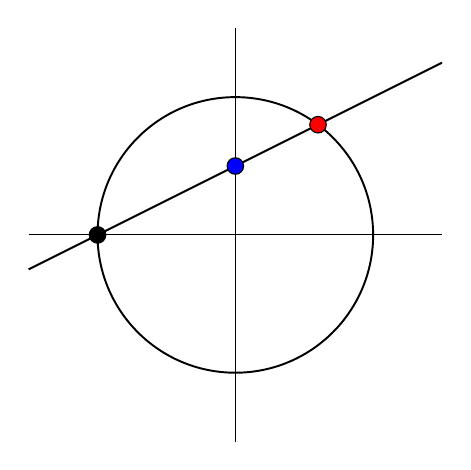
\begin{tikzpicture}[scale=1.75]
	\draw (-1.5,0) -- (1.5,0);
	\draw (0,-1.5) -- (0,1.5);

	\draw[line width=0.7] (-1.5,-0.25) -- (1.5,1.25);
	\draw[line width=0.7] (0,0) circle (1);
	
	\draw[fill=black] (-1,0) circle (0.06);
	\draw[fill=blue] (0,0.5) circle (0.06);
	\draw[fill=red] (0.6,0.8) circle (0.06);
	\end{tikzpicture}
	\] 
How would you go about doing this if it were the point $(0, 1)$ and you were projecting onto the line $y= -x$? \pspace

\problem Repeat the previous problem using the point $(0, 1)$ and projecting onto the $x$-axis to find the parametrization of (almost all) points on the circle. You may recall that $\displaystyle \int \sec \theta \;d\theta= \ln|\sec \theta + \tan \theta| + C$. Use the parameterization of the circle you just found to prove that this integral is correct. \pspace

\problem During the talk, it was claimed that there are no rational solutions to $x^2 + y^2= 3$. Prove this fact. [Hint. Assume there were a rational solution, clear denominators, then work modulo 4.] \pspace

\problem Can there be infinitely many solutions to $y^2 + y= x^5 + x^3 + x$? Explain. \pspace

\problem Show that 13 cannot be written as the sum of three cubes, i.e. there are no rational numbers $x, y, z$ with $x^3 + y^3 + z^3= 13$. [Hint: Assume there is a solution, clear denominators, and work modulo 9.] Can you find infinite families of numbers which are not the sum of three rational cubes? \pspace

\problem K. Mahler proved in 1936 that there are infinitely many expressions of 1 as the sum of three cubes by taking $x= 9b^4$, $y= 3b - 9b^4$, and $z= 1 - 9b^3$. Verify this fact and find an example of such an expression. \pspace

\problem Suppose you found a rational elliptic curve $E$ with three distinct points of infinite order. Moreover, you know there exists a point of order 2 and 5. What is the structure of the elliptic curve as an abelian group? Explain. Furthermore, if you found a rational point $P$ on $E$ with $P, 2P, \ldots, 12P \neq \mathcal{O}$, what must the order of $P$ be? Explain.

\end{document}